\hypertarget{sec:dsac-composition-platform}{%
\chapter{Model-driven Composition Application}\label{sec:dsac-composition-platform}}
The model-driven composition platform is the heart of our solution, designed to simplify the process of generating web \gls{api} mashup as domain specific situational tool. This chapter primary focused on \cref{ro:1}, aiming to provide domain experts with a usable method to develop domain-specific situational tool as composition platform. Firstly, the conceptual architecture of the platform is thoroughly reviewed in this chapter. Subsequently, two main tools namely Component Generator and \gls{dsac} Composer are reviewed in detail including the implementation steps and details of runtime environment. The evaluation of the Component Generator is presented in the final section.

\vspace{-10pt}
\hypertarget{sec:cp.analysis}{%
\section{Analysis}\label{sec:cp.analysis}}
\vspace{10pt}

With reference to objective \cref{ro:2}

\begin{quote}
Enable domain experts to develop an easy-to-use situational application and minimize reliance on software developers.
\end{quote}
this chapter proposes an approach to develop an easy-to-use situational decision making platform which serves as a tool to meet the transient needs of domain experts within their specific \gls{domain}. This contribution tackles the limited usability issue introduced in \cref{sec:problem}. 

As discussed in \cref{sec:introduction}, the decision-making procedures are becoming increasingly complicated and data-intensive. In such a situation, developing a situational application is primarily hindered by the complexity of web technologies, which necessitates a specific level of technical expertise. According to the assessment results presented in \cref{sec:sota.assessment}, composition methods focusing on EUD practices are the best candidates to alleviate these obstacles. In this chapter, the \gls{dsac} composition platform is introduced as well as the component generation module to convert \gls{api}s to platform-compliant components with a dedicated \gls{ui}. 
First, \cref{sec:dsac-cp:related-work} presents an analysis of related work to review existing state-of-the-art research. Following this, this chapter provides an overview of the conceptual architecture and platform implementation.

\vspace{-10pt}
\hypertarget{sec:dsac-cp:related-work}{%
\subsection{Related Work}\label{sec:dsac-cp:related-work}}
\vspace{10pt}

This section analyses the existing methods and solutions to develop a composition platform with a dedicated focus on usability for domain experts.
The service composition process can be analyzed from different perspectives depending on the use-case scenario. Each composite application addresses several core concerns, such as component access, control flow, data flow, or conversation management. These factors are crucial in  determining the suitable composition method \autocite{Lemos2015}. 


Composition methods can generally be classified into syntactic and semantic solutions. Syntactic solutions which include centralized and decentralized methods, focus only on the service description to plan the workflow, and execute the composition. In contrast, to increase the accuracy and performance, the semantic approaches leveraging the service’s semantic description to provide a goal-oriented compositions. Ontology-based API matching and knowledge graphs are some of the most effective methods in this category \autocite{Kim2016}.
In \gls{soa} paradigm, the web service composition involves several phases including, planning, discovery, selection, and execution \autocite{Rao2004}. In planning phase, the following two methods are the most common ones:

\textbf{Workflow-based} methods involves defining and managing a sequence of activities or tasks to achieve a specific goal. These methods are often used in business process management to orchestrate interactions between different services. They are primarily process-centric and typically follow a predefined sequence in static scenarios, which can not be useful in ever-changing environments. Examples of this method include \gls{bpmn}) \autocite{AlSedrani2016}.

In \textbf{AI Planning} methods, the web service composition is defined as a planning problem and addressed by AI techniques. These solutions are goal-oriented and automatically generate the final planning solution. The main objective in AI planning is to come up with a suitable sequence of web service that fulfill the end-user’s goal \autocite{AlSedrani2016}. To standardize the AI planning languages, the PDDL was proposed that can be an input for modern AI planners \autocite{Purohit2020}. Despite their advantages, AI planners often struggle with high complexity and inferior performance \autocite{Lee2015}.

In similar practices, the \gls{api} gateways like Kong  \footnote{\url{https://konghq.com/}} and Apigee \footnote{\url{https://cloud.google.com/apigee}} act as reverse proxies to manage and configure API interactions. However, these solutions require significant technical expertise for setup, configuration, and maintenance. Additionally, they lack domain-specific support, making them less accessible for domain experts.

%From the perspective of the \gls{eusc} paradigm, the composition models can be categorized into several types. The Language-based Compositions that includes script-based techniques used in programming-by-example, Flow-based methods are based on the application data or control flow. Form-based compositions are another group includes techniques such as spreadsheet-based and the final type is the interface-based methods such as \gls{wysiwyg} \autocite{Zhao2019}. 

\vspace{-15pt}
\hypertarget{sec:md-API-c}{%
\section{Model-driven \gls{api} Composition}\label{sec:md-API-c}}
\vspace{15pt}

This section introduced the conceptual architecture of the composition
platform. This platform is based on a model-driven development approach
aimed at facilitating the development of platform-independent
infrastructures for web mashup solutions. It provides \gls{api} service
composition tailored to the domain expert's
requirements. The conceptual architecture in Figure 5.1 illustrates the
different stages of the composition platform development process. Two
tools implementing this method, are \emph{Component Generator} and
\emph{\gls{dsac} Composer}. The Component Generator tasked with translating
\gls{rest}full \gls{api}s into \gls{dsac}-compliant components. The Component Generator
generates an ontology instance based on the \gls{api}'s specification to model
the \gls{api}'s data and communication schema. These instances play a crucial
role in the Composition Generation phase, where they are leveraged to
generate all possible component orchestrations to conceptualize the web
mashup solution. All model manipulations are performed as model
transformations to generate the component instances including the
executable code and the \gls{ui}.

\begin{figure}[hbt]
\hypertarget{fig:reference-architecture}{%
\centering
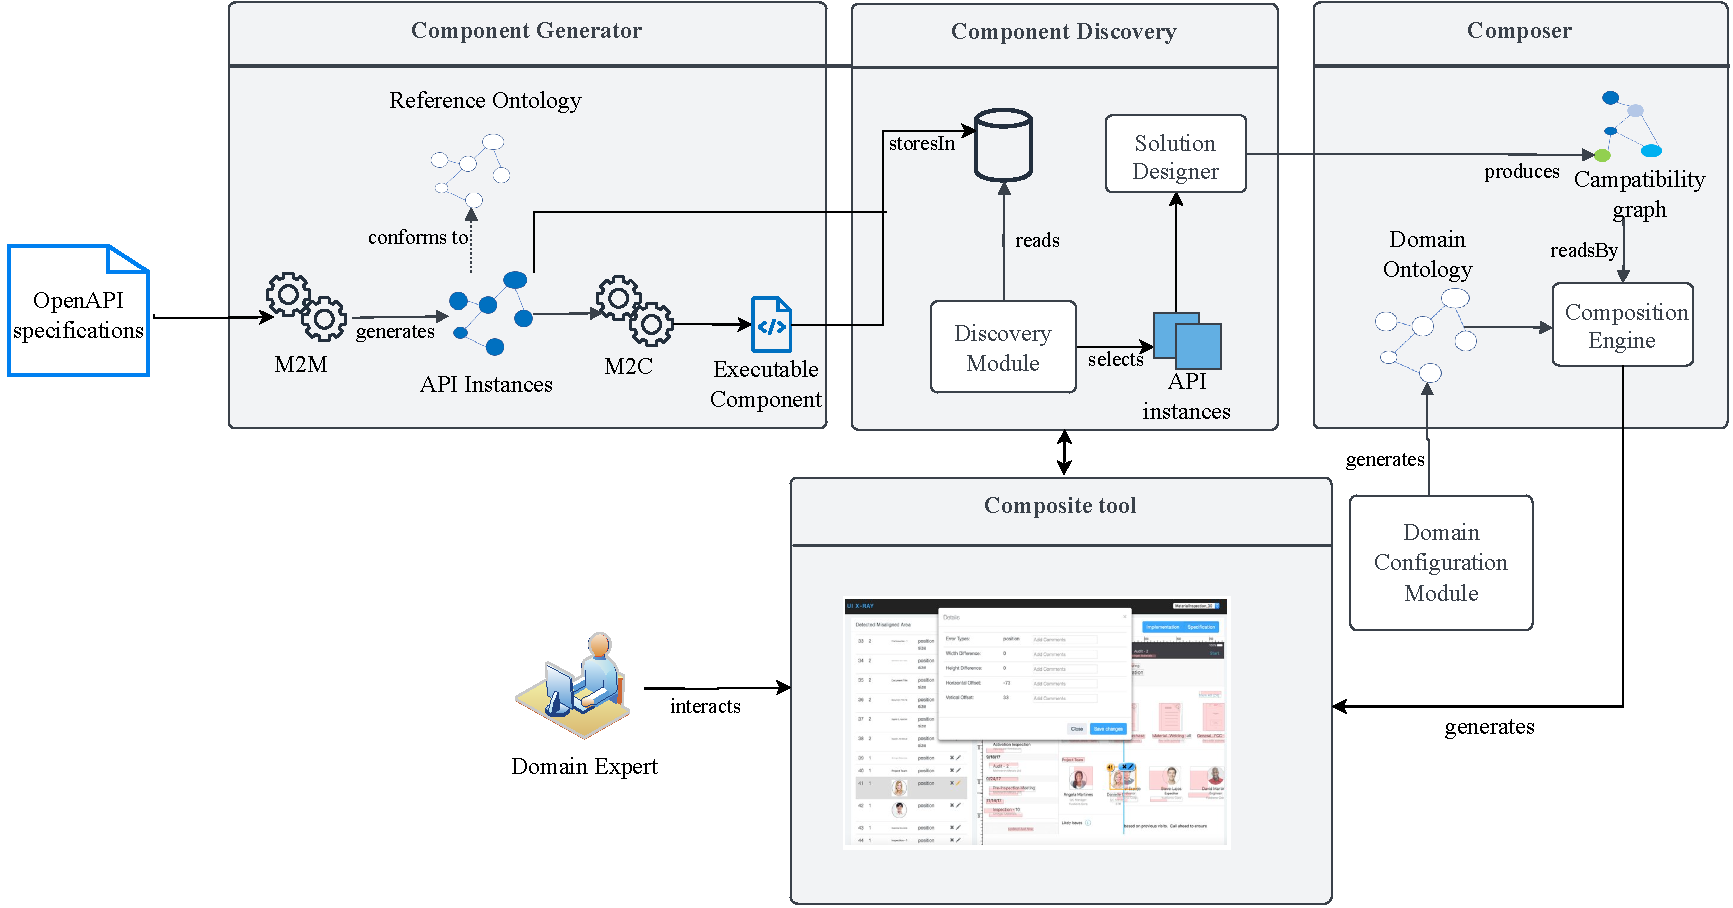
\includegraphics[width=0.85\textwidth]{../figures/MyFigures/ReferenceArch.drawio.pdf}
\captionsetup{justification=centering}
\caption{\gls{dsac} Platform Conceptual Architecture}\label{fig:reference-architecture}
}
\end{figure}
The component discovery module retrieves the potential components based on the component’s semantic description. A comprehensive overview of this module is provided in Chapter 6. 

The \gls{dsac} Composer responsible for compiling and deploying the composition solution and generating the executable code corresponding to the composition model and domain ontology. The composition model is executable as the run-time environment. The Domain Configuration module generates the domain layer and inject the domain knowledge into the platform (more details in Chapter 7).

The next two sections present the implementation details of the Component Generator and \gls{dsac} Composer tools in detail.

\hypertarget{sec:component-gen}{%
\section{Component Generator}\label{sec:component-gen}}
\vspace{15pt}

Components are the main building blocks of component-based development, defining the performance quality of the resulting platform. A limited number of components leads to inadequate resources to support domain experts in making informed decision. On the other hand, developing components from scratch is a time-consuming task that requires a certain level of expertise. Using existing component repositories is hindered by challenges such as format and data model incompatibility, as well as functional dependency \autocite{Tschudnowsky2016}. Therefore, it is crucial to support Component Developer and Repository Manager in generating and deploying \gls{dsac}-compliant components. 

\begin{figure}[hbt]
\hypertarget{fig:component-gen-diagram}{%
\centering
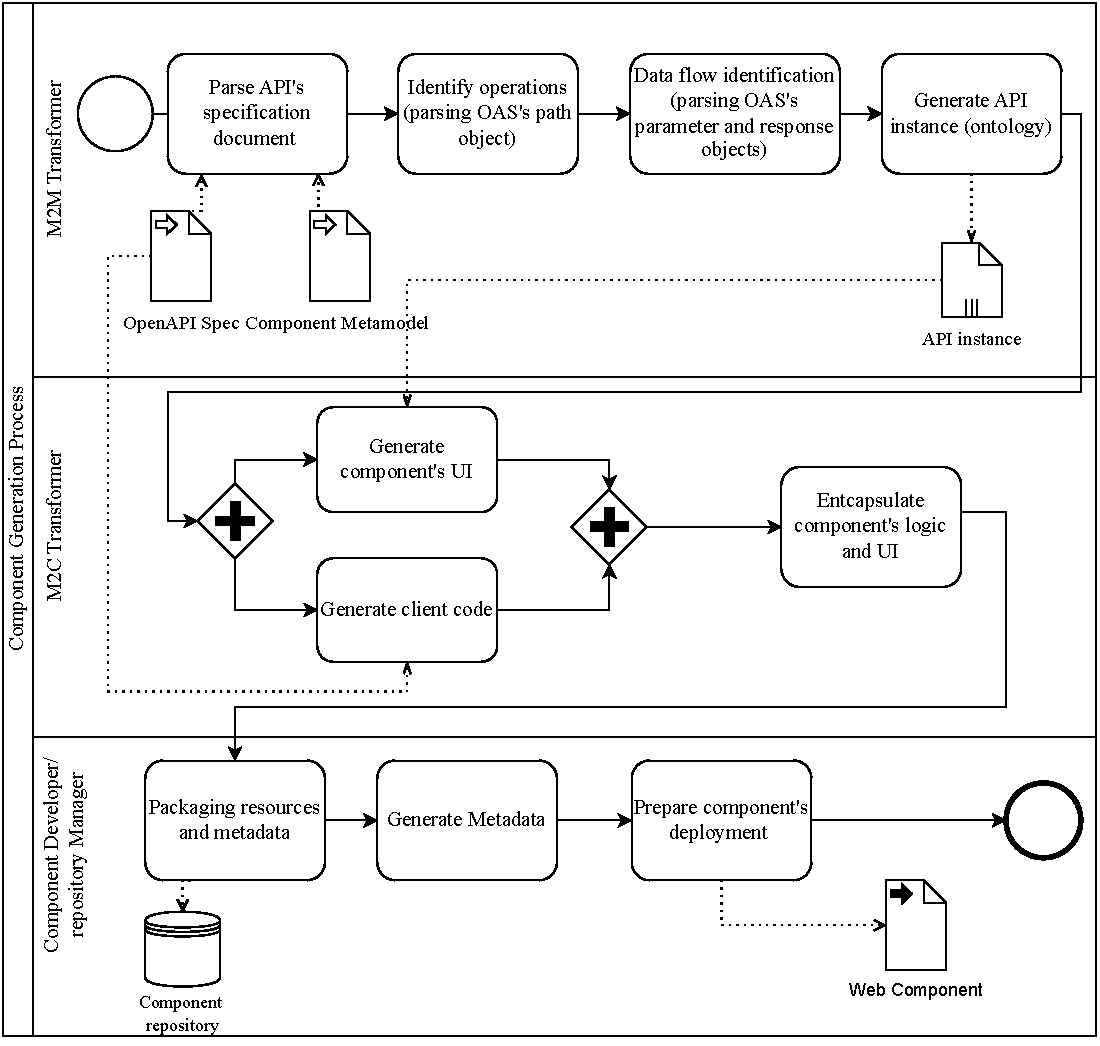
\includegraphics[width=0.85\textwidth]{../figures/MyFigures/ComponentGeneratorBPMN.drawio.pdf}
\captionsetup{justification=centering}
\caption{Component Generation Process Diagram}\label{fig:component-gen-diagram}
}
\end{figure}

The components in \gls{dsac} are full-fledged client-side applications
implemented using Web Components standard encapsulating HTML custom
elements. Each component has a unique name and a dedicated UI. The BPMN
diagram in Figure 5.2, illustrates these component generation process,
structured into three collaborative lanes: the \textbf{M2M Transformer},
performs a model-to-model transformation to generate API instance from
its specification; the \textbf{M2C Transformer}, focused on
model-to-code transformation for generating client-code and preparing
deployable components. The component developer and repository manager
are responsible for packaging, metadata generation, and repository
integration. The component's metadata includes a list of the component's
operation, which is used by Component Retrieve Engine during the
discovery phase (details in Section 6.4).

\vspace{-10pt}
\hypertarget{sec:api-instance}{%
\subsection{\gls{api} Instance Generation}\label{sec:api-instance}}
\vspace{10pt}

The first step involves deducting the component intermediate model from
REST APIs. The primary motivation for selecting REST APIs as the core
service style for this composition platform is their rapidly growing
popularity. Over the past decade, an increasing number of governmental
organizations and companies have invested in publishing their data and
services via REST APIs. Moreover, the number of registered APIs in
public repositories is increasing rapidly. This trend solidified REST
APIs as the backbone of web and mobile applications \autocite{Ed-douibi2017}.
Their widespread adaptation and availability make them ideal
building blocks for creating value-added applications and a promising
data source for situational applications \autocite{Zarei2021}.
To enable the systematic reuse of RESTful APIs, we consider the
OpenAPI\footnote{\url{https://www.openapis.org}} specification as the
choice of reference to describe REST APIs. This decision is supported by
several reasons: OpenAPI is an open and vendor-neutral specification,
widely supported by well-known software companies and providers such as
Google, Oracle, \gls{ibm}, and Microsoft, as well as a large community of users
\autocite{Karavisileiou2021}.

Generating API instances from their OpenAPI specifications is considered
a model-to-model transformation. The resulting instances conform to a
metamodel, which is an overall model defining the structure and
organization of elements and their properties within a given model
\autocite{Czarnecki2003}. \cref{fig:openapi-metamodel} shows the
OpenAPI metamodel as an intermediate representation of the OpenAPI 
specification, which is generated through the metamodeling approach. The
advantage of generating an OpenAPI-compliant intermediate model is to
facilitate the final component’s composition and manipulation.

\begin{figure}[hbt]
\hypertarget{fig:openapi-metamodel}{%
\centering
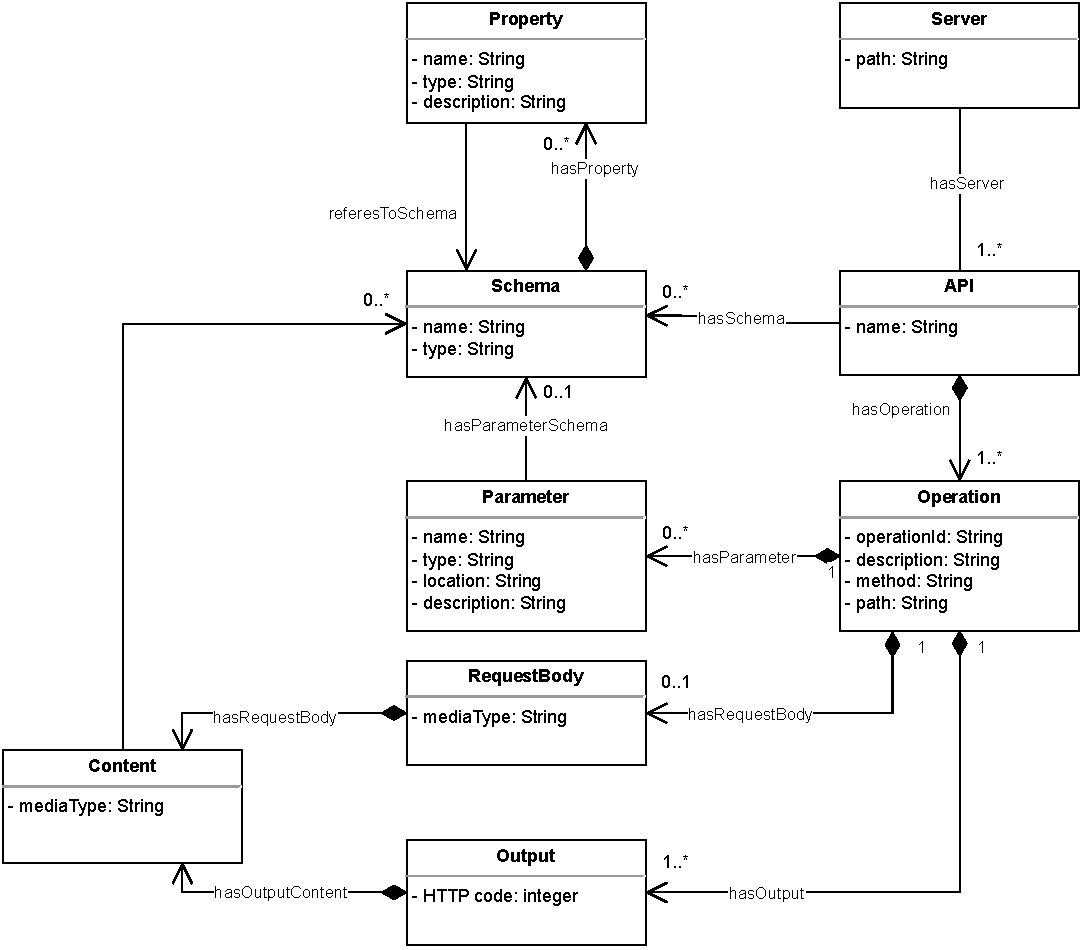
\includegraphics[width=0.85\textwidth]{../figures/MyFigures/openapi-metamodel.drawio.pdf}
\captionsetup{justification=centering}
\caption{OpenAPI Metamodel}\label{fig:openapi-metamodel}
}
\end{figure}

The root element of this metamodel is the \emph{API} class,
corresponding to the RESTful web API. This class includes references to
Operation (API services), Schema (API data structures), and hosting
Server. The operation class is described by the \emph{operationId},
description text, endpoint addresses known as \emph{paths}, and the \gls{http}
method to access the resources. Each operation can specify input data
using two mechanisms: parameter objects described by the
\emph{Parameter} class, or in the message body of the request described
by the \emph{RequestBody} class. The RequestBody must reference a
\emph{Content} class, describing inputs with different media types. The
data structure of the content is described by the \emph{Schema} class.
The API output is defined by the Response element in the OpenAPI
specification, which is modeled by the output class in the metamodel.
One of the core classes in this metamodel is Schema, which models the
API\textquotesingle s input/output data structure. Schema objects are
reusable and can be utilized by different operations. Each schema can
reference a number of \emph{Properties}.

To realize the automatic composition, the model-to-model transformation
is performed to generate the data schema, including the input and output
parameters, for each API. The data schema identifies the possible data
flow among APIs. Algorithms \hyperref[Algorithm5]{5.1} demonstrates API
instance generation. The inputs are the OpenAPI specification document
in \gls{json} format and the \gls{dsac} metamodel as an ontology. The algorithm
parses the OpenAPI document to model the data schema by instantiating
\emph{info}, \emph{servers}, \emph{paths,} and \emph{schemas} objects to
the \gls{dsac} metamodel classes. For each object, a corresponding individual
is created as well as its data and object properties. The OpenAPI
specification is scanned for all endpoints, known as paths. The Paths
object, which always begins with a forward slash (/), contains all the
API's supported operations. These operations match the \gls{http} method and
typically include a textual description that will be stored as the
operation's data property. Modeling API's input and output parameters
involves iterating thorough the parameter, request body, and response
objects. Listing 5‑1 shows an excerpt from the \gls{oas}
document of Interzoid API for weather forecast information.

\begin{lstlisting}[language=JavaScript, captionpos=t, caption=Snippet of the Paths Object from the Interzoid API’s Specification]
"paths": {
    "/getweatherzipcode": {
      "get": {
        "description": "Use a zip code to retrieve current weather information",
        "operationId": "getweatherzipcode",
        "parameters": [{
            "description": "Your Interzoid license API key. Register at www.interzoid.com/register",
            "in": "query",
            "name": "license",
            "required": true,
            "schema": {
              "type": "string"
            }
          },{
            "description": "Zip code for weather information",
            "in": "query",
            "name": "zip",
            "required": true,
            "schema": {
              "type": "string"
            }
          }]
      }
    }
  }
\end{lstlisting}

The parameters object, as defined in the parameters section of a path, is in array format with two mandatory fields: “in” to specify the parameter location (e.g., path, query, or header), and a case-sensitive “name” field. Additionally, the algorithm extracts the parameter type and description as a data property. To model the API’s output, Algorithm 5.3 scans the response object of each operation. Responses are named with an \gls{http} response code and has a mandatory description filed as the data property. Here only the successful responses (response code 200) are parsed as they represent the data schema of the output. The following listing shows an excerpt of the response object.

\begin{lstlisting}[language=JavaScript, captionpos=t, caption=Snippet of the Response Object from the Interzoid API’s Specification]
"responses": {
  "200": {
    "content": {
      "application/json": {
        "schema": {
          "properties": {
            "City": {
              "type": "string"
            },
            "Code": {
              "type": "string"
            },
            "Credits": {
              "type": "string"
            },
            "RelativeHumidity": {
              "type": "string"
            },
            "State": {
              "type": "string"
            }
          }
        }
      }
    }
  }}
\end{lstlisting}
The following algorithms describe the whole process.

\setlength{\algomargin}{2em} %

\begin{algorithm}
	\DontPrintSemicolon
	\KwIn{OpenAPI spec in JSON format as OAS,  API metamodel}
	\KwOut{API instance as the Ontology instance of the API}
	\begin{enumerate}
			\item 
			Open metamodel ontology;
			\item 
			Parse the info object of OAS:
			\begin{enumerate}
			  \def\labelenumii{\alph{enumii}.}
			  \item
			    \(API(info.title)\ \)create individual of class API
			  \item
			    Add \emph{description} and \emph{version} as API's data properties
			  \end{enumerate}
			\ForEach{URL in servers object of OAS object}
			{
				\begin{enumerate}
				  \def\labelenumii{\alph{enumii}.}
				  \item
				    \(Server(servers.url)\) create individual of class server for URL in
				    server property
				  \item
				    Add server as API's object property
				  \end{enumerate}
			}\label{endfor}
			
			
			\ForEach{path in paths object of OAS}
			{
				\ForEach{operation in paths}
				{
					\begin{enumerate}
					  \def\labelenumii{\alph{enumii}.}
					  \item
					    \(Operation ( operationId)\) create individual of class Operation
					  \item
					    Add operation as API's object property
					  \item
					    Add \emph{path}, \emph{method}, and \emph{description} as
					    operation's data properties
					  \item
				    If \emph{parameter} object is in operation or \emph{requestBody} is in
					    operation
					
					    \begin{enumerate}
					    \def\labelenumiii{\roman{enumiii}.}
					    \item
					      \(InputObject(operation,\ parameter,\ requestBody,\ APIInstance \). Refer to Algorithm 5.2.
					    \end{enumerate}
					    \item 
					    For responses in operation if response.code = 200
					    \begin{enumerate}
					    	\def\labelenumiii{\roman{enumiii}.}
					    	\item
					    	\(ResponseObject( operation,\ responses,\ APIInstance \). Refer to Algorithm 5.3.
					    \end{enumerate}
					  \end{enumerate}
					  
				}\label{endfor}
			
			}\label{endfor}
			
			\ForEach{\emph{schema} in \emph{components} object of OAS}{
				\begin{enumerate}
				  \def\labelenumii{\alph{enumii}.}
				  \item
				    \(Schema(schemaName)\) create individual of class Schema
				  \item
				    For each \emph{property} in \emph{properties} object of schema:
				
				    \begin{enumerate}
				    \def\labelenumiii{\roman{enumiii}.}
				    \item
				      \(Property(schemaName.property)\) create individual of class
				      property
				    \item
				      Add \emph{propertyType}, \emph{propertyName} and
				      \emph{propertyDescription} as the property data type.
				    \item
				      If property refers to another schema by ``\$ref'', then add the
				      reference to schema object.
				    \item
				      Add property as schema's object property.
				    \end{enumerate}
				  \end{enumerate}
			}\label{endfor}
			
			\item 
			Return the APIInstance
			
			\end{enumerate}
	\caption{API Instance Generation}\label{alg:api-instance-gen}
\end{algorithm}


\setlength{\algomargin}{2em} %
\begin{algorithm}
	\DontPrintSemicolon
	\KwIn{Operation object, parameter object, requestBody object and APIInstance}
	\KwOut{Ontology instance with parameter and/or request body}
	\begin{enumerate}
	\item 
	\ForEach {\emph{parameter} in \emph{parameters} object in operation}
	{
		\begin{enumerate}
		\def\labelenumi{\alph{enumi}.}
		\item
		  create the individual of class parameter and add it to APIInstance.
		\item
		  Add \emph{parameterType}, \emph{parameterName},
		  \emph{parameterDescription} and \emph{parameterLocation} as the
		  parameter's data property.
		\end{enumerate}
	}\label{endfor}
	
	\If {\emph{requestBody} is not empty}{
	\begin{enumerate}
	\def\labelenumi{\alph{enumi}.}
	\item
	  Creates the individual of class requestBody and add it to
	  APIInstance.
	\item
	  For each request body \emph{contentType}: ~create the individual of
	  class Content.
	\item
	  For schema in \emph{content} object:
	  \begin{enumerate}
	  \def\labelenumi{\roman{enumi}.}
	  \item
	    If there is a referenced schema in content object, then add schema
	    instance from the schemas extracted in Algorithm 5 step 6.
	  \item
	    If properties in schema object: 
	    \begin{enumerate}
	    \def\labelenumi{\arabic{enumi}.}
	    \item
	      Create individual of class property
	    \item
	      Add \emph{propertyType}, \emph{propertyName} and
	      \emph{propertyDescription} as the property data type.
	    \end{enumerate}
	    
	  \end{enumerate}
	  
	\end{enumerate}
	
	}
	\item 
	Return APIInstance.
	\end{enumerate}
	
\caption{Input Object Extraction}\label{alg:api-instance-input}
\end{algorithm}


\setlength{\algomargin}{2em} %
\begin{algorithm}
	\DontPrintSemicolon
	\KwIn{OpenAPI spec in JSON format as OAS,  API metamodel}
	\KwOut{API instance as the Ontology instance of the API}
	\begin{enumerate}
		\item 
		\ForEach {\emph{response} in \emph{responses}}
			{
				\begin{enumerate}
				  \def\labelenumii{\alph{enumii}.}
				  \item
				    If response code is "200" or "default" then, creates the output
				    individual and add it to APIInstance
				    \(Output(operationId."output")\)
				  \item
				    Add \emph{outputDescription} as the output's data property.
				  \item
				    \(Content\ (operationId."output".Mediatype)\) create the individual
				    of class Content.
				  \item
				    \ForEach{content type}
				    {
				    	 \begin{enumerate}
				    					    \def\labelenumiii{\roman{enumiii}.}
				    					    \item
				    					      If there is a referenced schema is in content object, then add
				    					      schema instance from the schemas extracted in Algorithm 5 step 6.
				    					    \item
				    					      If properties in schema object:
				    					
				    					      \begin{enumerate}
				    					      \def\labelenumiv{\arabic{enumiv}.}
				    					      \item
				    					        \(Property(schemaName.property)\) create individual of class
				    					        property.
				    					      \item
				    					        Add \emph{propertyType}, \emph{propertyName} and
				    					        \emph{propertyDescription} as the property data type.
				    					      \end{enumerate}
				    					    \end{enumerate}
				    }\label{endfor}		   
				  \end{enumerate}
			
			}\label{endfor}
	\item 
	Return APIInstance
		
\end{enumerate}
	
	
	\caption{API’s response object as the output}\label{alg:api-instance-response}
\end{algorithm}


\vspace{-10pt}
\hypertarget{sec:clientCode-gen}{%
\subsection{Component’s Client Code Generation}\label{sec:clientCode-gen}}
\vspace{10pt} 	

To generate executable components, a model-to-code transformation is performed to generate the component’s client code and UI. This transformation relies on the API instance produced by the M2M transformation. The generation process consists of three steps: a) client code generation based on the API’s operations, b) encapsulating the client code and \gls{ui} into web components, and c) packaging the content resources and metadata into folders. During the first step, the client code for invoking the API and consuming its service is generated automatically, with the help of the OpenAPI Generator library \footnote{\url{https://openapi-generator.tech/}}. OpenAPI Generator is an open-source project for generating API clients from OpenAPI specification documents in various programming languages \autocite{Springborg2022}. Figure 5.4 shows the folder structure of the generated client code for Interzoid API:

\begin{figure}[hbt]
\hypertarget{fig:openapi-generator}{%
\centering
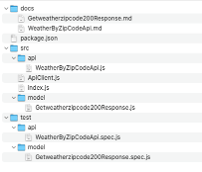
\includegraphics[width=0.85\textwidth]{../figures/MyFigures/Picture 1.png}
\captionsetup{justification=centering}
\caption{Example of OpenAPI Generator File Structure}\label{fig:openapi-generator}
}
\end{figure}

The ApiClient.js file contains all the necessary methods for executing
\gls{http} requests based on the specified operations. In other words, the
ApiClient file is an abstract layer to encapsulates the API's
communication details. Throughout the next step, the actual component is
generated by wrapping the API client code within a custom web component
using the Google Polymer\footnote{\url{https://polymer-library.polymer-project.org/}.
  This library is now in the maintenance mode. The new developments are
  available as Lit package in \url{https://lit.dev/}} framework. Web
component is a W3C standard including a set of features that allows
encapsulation of complex services to present a consistent interface and
operation. Web components promote the reusability and interoperability
of \gls{html} elements \autocite{Yang2002a}, and according to \autocite{Rojas2021} Polymer web components are supported by all the major web browsers
and used widely by leading companies such as Google and YouTube.

Moreover, applying component-based techniques promotes separation of
concern, advising developers to decompose an application into
well-isolated ``concerns'' which can be addressed in separated modules
with minimal overlap. Mechanisms such as modulization and encapsulation
are the best practices for applying the separation of concerns principle
\autocite{Piessens2002}.

Each \gls{dsac} component is structured with two layers of Business Logic and
Presentation. The Business logic layer runs the component logic and
operations by making \gls{html} requests, binding data, and error handling.
The presentation layer is in charge of the component's visual
representation by encapsulating the \gls{html} and CSS elements. To generate
the component's \gls{ui} (presentation layer) Algorithm 5.4 is applied as follow:

\setlength{\algomargin}{2em} %
\begin{algorithm}
	\DontPrintSemicolon
	\KwIn{OpenAPI specification document in \gls{json} format as \gls{oas}}
	\KwOut{<template> element to added to the component}
	\begin{enumerate}
	\item 
	\ForEach {\emph{param} in \emph{parameters} object of operation and
	  \emph{requestBody}}
	{
		\begin{enumerate}
		\def\labelenumii{\alph{enumii}.}
		  \item
		    Add \emph{\textless label for="\{param{[}"name"{]}\}"
		    id="name\_\{param{[}"name"{]}\}"\textgreater\{\{name\_\{param{[}"name"{]}\}\}\}\textless/label\textgreater{} 
		    \emph{\textless input type="text" id="\{param{[}"name"{]}\}"
		    name="\{param{[}"name"{]}\}"
		    value="\{\{\{param{[}"name"{]}\}\}\}"/\textgreater{}}to
		    \textless template\textgreater{} element}
		\end{enumerate}
	}\label{endfor}
	
	\item 
	\ForEach {\emph{content} and \emph{properties} of \emph{response} with
	  code "200"}{
	  \begin{enumerate}
	    \def\labelenumii{\alph{enumii}.}
	    \item
	      Add \emph{\textless p\textgreater\{prop\}:\textless span
	      id="\{prop\}"\textgreater\{\{\{prop\}\}\}\textless/span\textgreater\textless/p\textgreater{}}
	      to the \textless template\textgreater{} element
	    \end{enumerate}
		}\label{endfor}
	
	\item 
		Return <template>
	\end{enumerate}
	
\caption{Component UI template Generation}\label{alg:ui-gen}
\end{algorithm}

As indicated in Algorithm 5.4
\emph{label} and \emph{input} elements have unique Ids to match the
unique input for each parameter. An important aspect of building web components is data binding, which
synchronizes the component's model and the view in terms
of transferred data. Generally, two types of binding patterns are
prevalent: one-way and two-way binding. In one-way binding, data flows
in only one direction, either from the view to the
component's model or vice versa. This pattern is
suitable for static components whose internal state should not be
altered by user interaction. Conversely, two-way binding enables the
creation of interactive components, allowing both the model and view to
be changed in real time. This technique ensures the development of
dynamic and responsive components \autocite{Rojas2021}.

In this work the two-way binding pattern is implemented by using event
listeners (also referred to as observers in Polymer) and property
setters. The use of double curly braces in Algorithm 5.4 establishes a binding between a property and
an input element.
To facilitate intercomponent communication, the pub/sub pattern is
implemented. Components subscribe to events by defining an event
listener for each input. On the other hand, whenever a component
produces output, an event is emitted that can be consumed by components
subscribed to that specific topic.

To be able to use the client code in the browser the generated module
should be bundled in java script and deployed during the composition
generation step by the \gls{cd} and \gls{rm}.

\hypertarget{sec:dsac-composer}{%
\section{\gls{dsac} Composer}\label{sec:dsac-composer}}
\vspace{15pt}

The \gls{dsac} composer is responsible for producing~the final composite
application as a web-based runtime environment. This module contains
the \emph{Composition Engine}, which generates the composition model
(cf. Section 4.2.2) using the \emph{Compatibility Graph}. This graph was
produced by the Solution Designer (refer to Section 6.5 for specifics)
and outlines the Communication Configuration within the composition
model, dictating inter-component channels. Another module of \gls{dsac}
Composer is the \emph{Composition Compiler} which compiles the resultant
composition model into executable code and deploys the final mashup
solution. Once the deployment is successful, the Composition Engine
notifies the domain expert to inform them that the process is complete.
Following \gls{bpmn} diagram presents the workflow of this process.

\begin{figure}[hbt]
\hypertarget{fig:composition-gen}{%
\centering
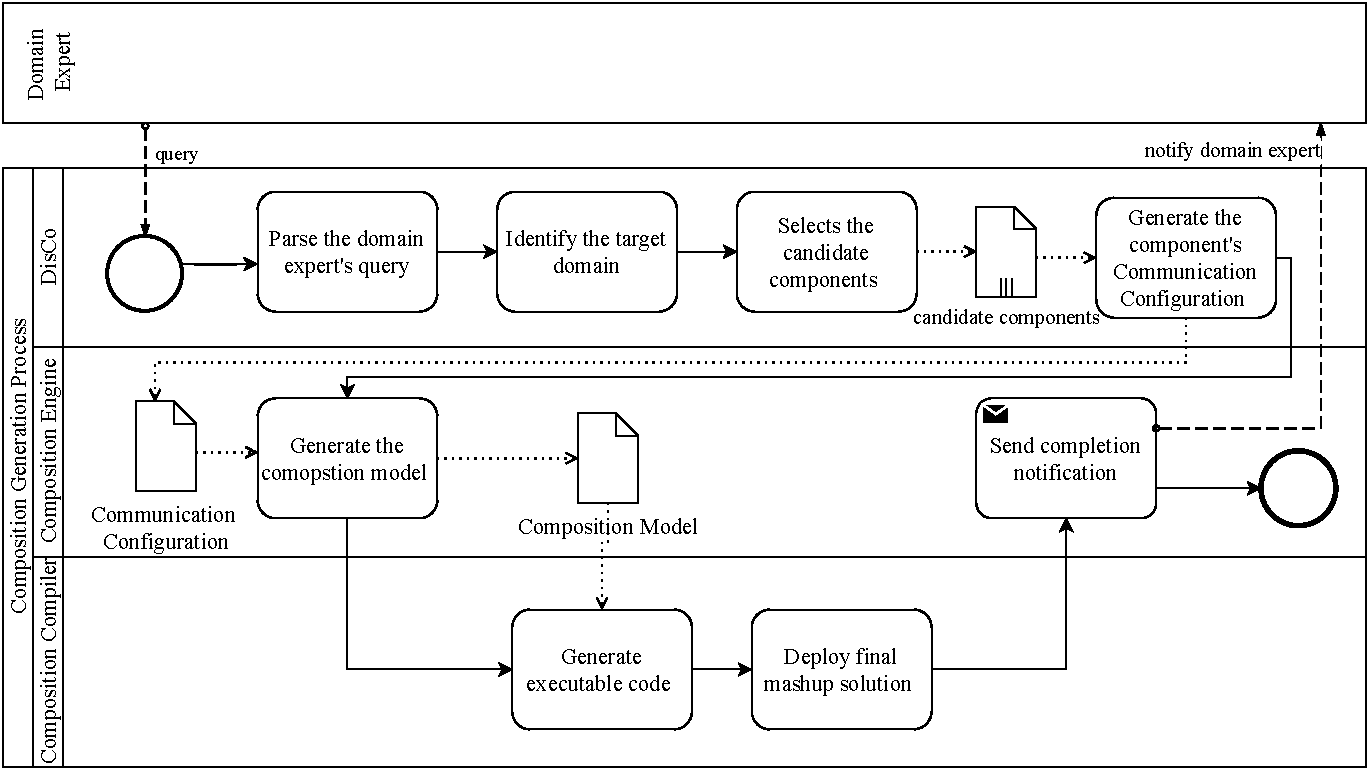
\includegraphics[width=0.85\textwidth]{../figures/MyFigures/CompositionBPMN.drawio.pdf}
\captionsetup{justification=centering}
\caption{BPMN Diagram of \gls{dsac} Composition Generation Process}\label{fig:composition-gen}
}
\end{figure}

To provide a comprehensive overview, the diagram also includes the \gls{disco}, responsible for discovering and retrieving the component candidates. This tool is introduced in Chapter 6. The composition model is in \gls{json} format and include the selected component’s instances. This model contains the layout specifications and the data flow abstract syntax.

\vspace{-10pt}
\hypertarget{sec:composition-imp}{%
\subsection{Composition Implementation}\label{sec:composition-imp}}
\vspace{10pt}

To efficiently implement the \gls{dsac} composition, we present a client/server architecture. Client-side hosts the \gls{ui} within a web browser, allowing users to interact with the \gls{dsac} mashup. On the server side, the executable representation of the final mashup is generated, and the external API interactions are managed. The following figure illustrates this architecture and its building elements.

\begin{figure}[hbt]
\hypertarget{fig:composition-arch}{%
\centering
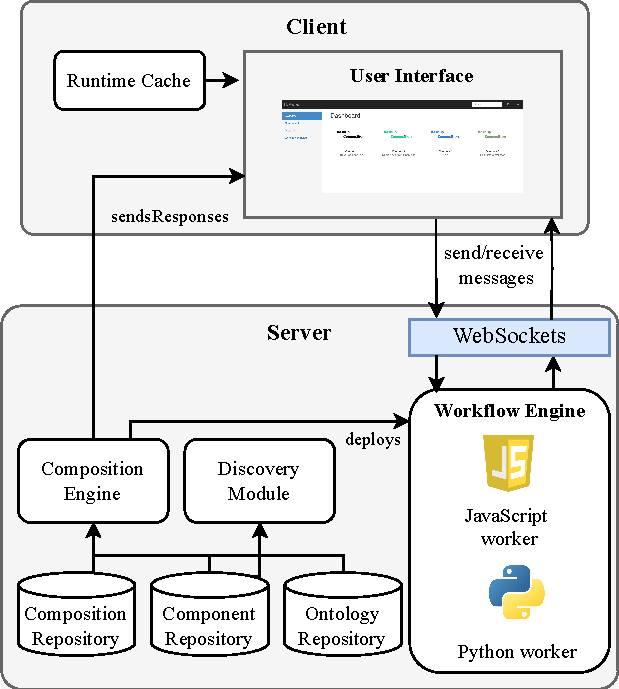
\includegraphics[width=0.85\textwidth]{../figures/MyFigures/Client_server.drawio.pdf}
\captionsetup{justification=centering}
\caption{\gls{dsac}‘s Client/Server Architecture}\label{fig:composition-arch}
}
\end{figure}
This architecture is implemented~on top of several technologies.
JavaScript and Google libraries like Polymer are employed on the client
side for \gls{ui} implementation. On the server side, two-way communication
channels with the client are established using WebSocket. The WebSocket
protocol provides reliable and efficient communication sessions for
sending and receiving messages in an event-driven manner. The reason for
choosing WebSocket over \gls{http} polling or long-polling techniques is the
low-latency communication and enhanced efficiency by eliminating the
overhead of \gls{http} headers. The inter-component communication is also
performed through WebSocket, where the compatibility graph is mapped
into WebSocket's connections \autocite{Kotevski2011}.

Another server-side module is the \emph{Workflow Engine}, tasked with
orchestrating the interaction and integration of web mashup components.
Each workflow comprises distinct tasks, including initializing the user
interface, registering, and executing components, and managing
communications and errors. These tasks are carried out by individual
workers concurrently or sequentially based on the composition model. The
event-driven Workflow Engine is implemented in ~Node.js and runs two
worker threads:~one~for executing JavaScript code and another for
running Phyton codes primarily employed for the Domain Configuration
Module.

Composition Engine can store and read data form composition and
component repositories and send notifications to the \gls{ui}.


\vspace{-10pt}
\hypertarget{sec:dsac-mashup-solution}{%
\subsection{\gls{dsac} Mashup Solution}\label{sec:dsac-mashup-solution}}
\vspace{10pt}

After successful composition generation, the mashup is ready for execution and the user is notified about the end of the deployment. The \gls{dsac} platform is implemented as a web mashup using Vanilla \gls{js}. To optimize the tool’s runtime performance in terms of response time, we implemented a caching mechanism to reduce the excessive request calls to the components. We used the Service Worker in JavaScript to cache the API responses. The Service Worker is registered during the runtime and implements the caching logic by caching the API's endpoints. The Service Worker then intercepts fetch requests made by the mashup tool and serves responses from the cache if available or fetches them by making the API request.

\vspace{-15pt}
\hypertarget{sec:cp.evaluation}{%
\section{Evaluation}\label{sec:cp.evaluation}}
\vspace{15pt}

This section outlines the evaluation process for the Component Generator introduced in this chapter, focusing on the requirements detailed in \cref{sec:requirements}. The evaluation for \gls{dsac} Composer, as a part of the overall assessment, is presented in Chapter 8 to comprehensively evaluate the tool's performance.

%\vspace{-10pt}
\hypertarget{sec:cp.evaluation.cg}{%
\subsection{Component Generator Evaluation }\label{sec:cp.evaluation.cg}}
\vspace{10pt}

The \textbf{Semi-Automation} requirement, outlined in \cref{pr:1}, emphasizes the active involvement of end users throughout the development and deployment phases. Although the model-to-model and model-to-code processes operate automatically, the responsibility for deployment and maintenance rests with component developers and repository managers. This involvement ensures efficient integration and management of components within the solution framework. Therefore, this requirement is considered as fully satisfied.

The \textbf{Systematic Reuse} requirement ensures efficient time and cost utilization by promoting the reuse of software artifacts. The component generator uses the OpenAPI specification of existing REST \gls{api}s adhering to the OpenAPI standard. Therefore, developers gain access to a vast ecosystem of well-documented and standardized \gls{api}s covering various functionalities and services. As a result, this requirement is considered fully satisfied. 

The \textbf{Effectiveness} requirement refers to the degree to which the solution achieves its intended objectives. The solution is considered to be effective if it delivers the desired situational solution for the problem it was designed to address. Evaluating the effectiveness of a tool involves assessing its accuracy, completeness, and efficiency \autocite{Semiawan2021}. In evaluating the Component Generator tool, completeness refers to how well it covers all basic API’S operations. Both completeness and accuracy are crucial to prevent generating numerous false positives (complete generated components with incorrect operations).

To this measure, 20 \gls{api}s are randomly downloaded from public OpenAPI repositories. These \gls{api}s are selected from the top five domains listed in ProgrammableWeb. Components are generated according to the \gls{api}’s document and reviewed manually after each transformation round. The completeness is calculated as 90\% indicating that the tool failed to generate two components. The accuracy rate is calculated as 80\% by manually comparing the generated component’s client code and \gls{ui} with the OpenAPI spec document. 

\vspace{-15pt}
\hypertarget{sec:cp.summary}{%
\section{Summary}\label{sec:cp.summary}}
\vspace{10pt}

This chapter introduced the \gls{dsac} platform, designed for domain experts to develop situational solutions in the form of web mashups. To this end, two tools were introduced, Component Generator to create components aligned with the model outlined in \cref{sec:solution}. Each component encapsulates functionalities of an  \gls{api} and presents its \gls{ui} as a web component. The second tool, the \gls{dsac} Composer, produces the composition model and compiles it into the executable code. The evaluation of the component generator module revealed acceptable performance and a high level of usability. The next two chapters present further extensions of the composition platform, with Chapter 6 focusing on the tools for component discovery and composition generation processes, and Chapter 7 addresses objectives related to domain specificity.